\section{Nachhaltigkeit}

Im Sinne einer ressourcenschonenden Entwicklung, angelehnt an das 3R-Prinzip (Reduce, Reuse, Recycle) sowie das 12. Ziel für nachhaltige Entwicklung der Vereinten Nationen („Nachhaltige Konsum- und Produktionsmuster sicherstellen“), wurde die Wiederverwendbarkeit von Bauteilen gezielt berücksichtigt. Die Grundplatte des Prototyps aus PREN1 wurde so konstruiert, dass sie modular erweiterbar ist. Zusätzliche Bohrungen und Nuten konnten während der Entwicklung fortlaufend eingebracht werden, ohne dass eine neue Platte gefertigt werden musste. Die Nachbearbeitung mittels Laserschneidmaschine verlief dabei ohne technische Probleme. Dadurch konnte der Materialeinsatz auf eine einzige Grundplatte beschränkt und die Entstehung von Abfall minimiert werden. Eine Übersicht der verschiedenen Bearbeitungszustände ist in Abbildung \ref{fig: Weiterentwicklung der Grundplatte} dargestellt.


\begin{figure}[H] % oder [htbp]
    \centering
    \begin{subfigure}[b]{0.45\textwidth}
        \centering
        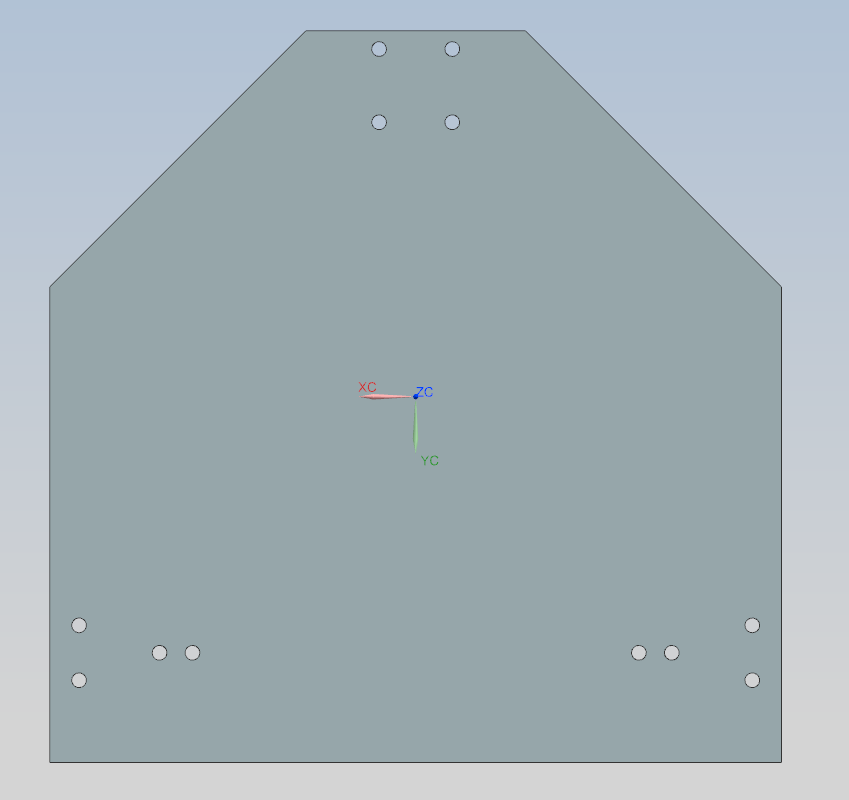
\includegraphics[width=\linewidth]{assets/MT/Grundplatte_V0.png}
        \caption{Grundplatte V0}
    \end{subfigure}
    \hfill
    \begin{subfigure}[b]{0.45\textwidth}
        \centering
        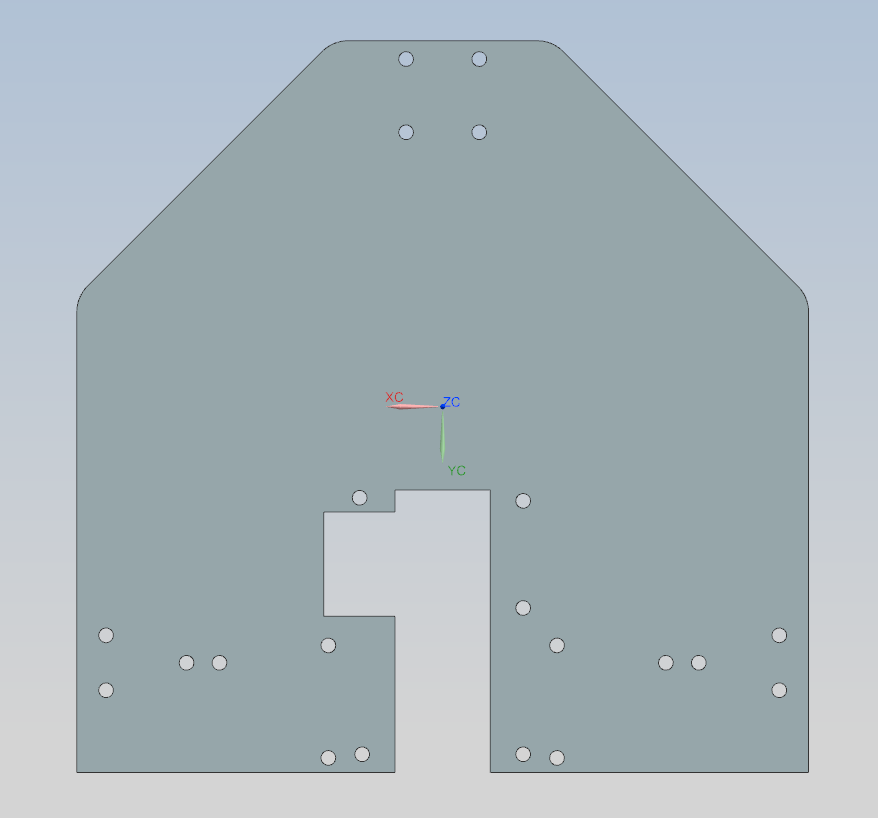
\includegraphics[width=\linewidth]{assets/MT/Grundplatte_V1.png}
        \caption{Grundplatte V1}
    \end{subfigure}

    \vspace{0.5cm}

    \begin{subfigure}[b]{0.45\textwidth}
        \centering
        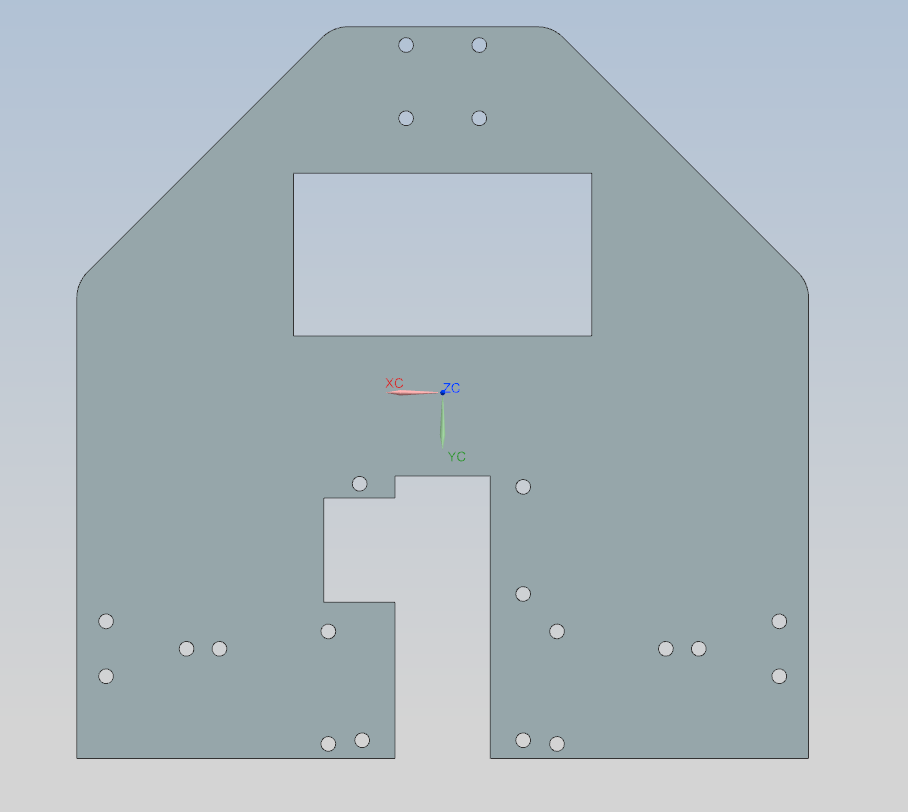
\includegraphics[width=\linewidth]{assets/MT/Grundplatte_V2.png}
        \caption{Grundplatte V2}
    \end{subfigure}
    \hfill
    \begin{subfigure}[b]{0.45\textwidth}
        \centering
        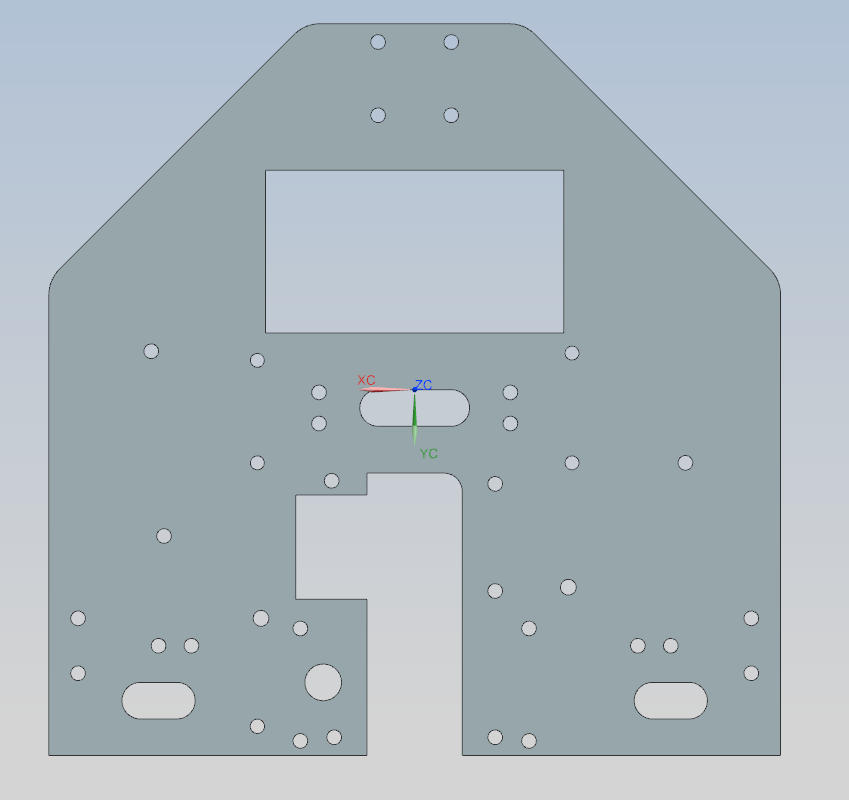
\includegraphics[width=\linewidth]{assets/MT/Grundplatte_V3.png}
        \caption{Grundplatte V3}
    \end{subfigure}
    \caption{Weiterentwicklung der Grundplatte}
    \label{fig: Weiterentwicklung der Grundplatte}
\end{figure}


\section{Ökobilanz und Materialanalyse}

\subsection{Betrachtung hinsichtlich Ökobilanz}
% Beschreibung des Gesamtgewichtes und der drei größten Material-Positionen
Das Gesamtgewicht des Fahrzeugs beträgt [\textbf{Gesamtgewicht}]. In folgender Tabelle werden die drei grössten Material-Positionen in Kilogramm und Prozent des Gesamtgewichtes aufgelistet, gefolgt von einer Beschreibung der Recyclingfähigkeit, Entsorgung und/oder Abfallbehandlung dieser Materialien.

\begin{table}[h]
\centering
\caption{Material-Positionen nach Gewichtsanteil}
\begin{tabular}{l c c p{5cm}}
\toprule
Material & Gewicht  & Anteil (\%) & Beschreibung der Recyclingfähigkeit/Entsorgung \\
\midrule
\acrshort{mdf} & 0.166kg & [AUSRECHNEN!35\%] & Recycelbar aber schwierig \\
\acrshort{pla} & 0.252 kg & [AUSRECHNEN!\%] & Gut Recycelbar \\
Batterie & 0.202 KG & [AUSRECHNEN!40\%] & Recyceln möglich aber ist teuer \\
\bottomrule
\end{tabular}
\end{table}

\subsection{Nachhaltig-kritischste Materialien}
% Auflistung und Beschreibung der nachhaltig-kritischsten Materialien
Im Folgenden werden mindestens drei der nachhaltig-kritischsten Materialien, die im Fahrzeug verbaut sind, aufgelistet. Für jedes Material wird erläutert, warum es nicht nachhaltig ist, und es werden mögliche Massnahmen zur Vermeidung vorgeschlagen.

\begin{itemize}
    \item \textbf{Material 1:} \acrfull{mdf} \\
          \textit{Grund der mangelnden Nachhaltigkeit:} Hoher Energieaufwand und vergleichbar hoher Leimanteil  \\
          \textit{Vermeidungsstrategie:} Leimholzplatten mit weniger Leimanteil oder Massivholzplatten verwenden. Ökolgisch zertifiziertes MDF ist nachhaltiger
          
    \item \textbf{Material 2:} Lithium in der Batterie \\
          \textit{Grund der mangelnden Nachhaltigkeit:} Lithium ist umweltschädlich bei der Herstellung. Abbau und Raffinerie benötigt viel Energie und Wasser und setzt Schadstoffe frei. \\
          \textit{Vermeidungsstrategie:} Lithium für Batterien ist praktisch nicht vermeidbar wenn eine Batterie benötigt wird. Der Herstellungsprozess kann jedoch umweltfreundlicher gestaltet werden
          
    \item \textbf{Material 3:} Kupfer in Kabel \\
          \textit{Grund der mangelnden Nachhaltigkeit:} Kupfer ist umweltschädlich bei der Herstellung. Abbau und Raffinerie benötigt viel Energie und Wasser und setzt Schadstoffe frei. \\
          \textit{Vermeidungsstrategie:} Kabel und Leitungen von Hersteller beziehen welche ausschliesslich recycletes Kupfer verwenden.
\end{itemize}